% Foliensatz: "AFu-Kurs nach DJ4UF" von DK0TU, Amateurfunkgruppe der TU Berlin
% Lizenz: CC BY-NC-SA 3.0 de (http://creativecommons.org/licenses/by-nc-sa/3.0/de/)
% Autoren:
% Felix Baum <baum@campus.tu-berlin.de>
% Korrekturen:
% Lars Weiler <dc4lw@darc.de>

preamble.dk0tu.tex
\subtitle{Technik 15: \\
  Sender- und Empfängertechnik \\[2em]}
\date{Stand 18.09.2017}
 \begin{document}

\begin{frame}
    \titlepage
    \vfill
    \begin{center}
        \ccbyncsaeu\\
        {\tiny This work is licensed under the \em{Creative Commons Attribution-NonCommercial-ShareAlike 3.0 License}.}\\[0.5ex]
         \tiny Amateurfunkgruppe der Technische Universität Berlin (AfuTUB), DKØTU
         %\includegraphics[scale=0.5]{img/DK0TU_Logo.pdf}
    \end{center}
\end{frame}


\section*{Einleitung}

\begin{frame}
  \frametitle{Was ist das?}
  \begin{center}
    \begin{figure}
      \includegraphics[width=.95\textwidth,height=.75\textheight,keepaspectratio]{e15/bitx.png}
      \caption{Schaltplan von \ExternalLink\url{http://www.phonestack.com/farhan/bitx.html}}
    \end{figure}
  \end{center}
\end{frame}

\begin{frame}
  \frametitle{In freier Wildbahn}
  \begin{itemize}
    \item Wo findet man Sender?
    \item Wo findet man Empfänger?
  \end{itemize}
\end{frame}

\begin{frame}
  \frametitle{Funktion}
  \begin{center}
    \begin{figure}
      \includegraphics[width=1\textwidth,height=.75\textheight,keepaspectratio]{e15/TRX-superSimple.png}
      \attribcaption{Steps in a signal communications system}{Brews ohare}{https://en.wikipedia.org/wiki/File:Signal_processing_system.png}{\ccbysa}
    \end{figure}
  \end{center}
\end{frame}

\section*{Sender}

\begin{frame}
  \frametitle{Sender -- Blockschaltbild}
  \begin{center}
    \begin{figure}
      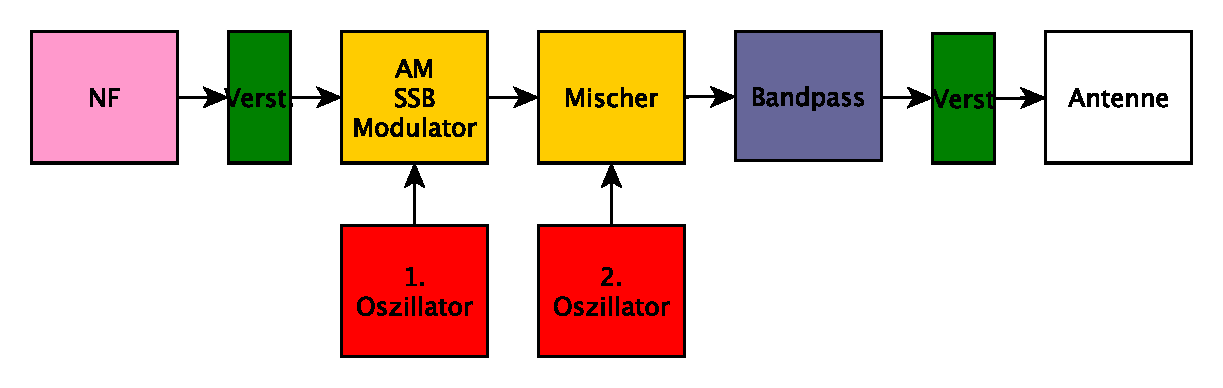
\includegraphics[width=1\textwidth,height=.75\textheight,keepaspectratio]{e15/ssb-trx-bsb.pdf}
      \caption{von DB4UM}
    \end{figure}
  \end{center}
\end{frame}

\begin{frame}
  \frametitle{Sender}
  \begin{center}
    \begin{figure}
      \includegraphics[width=.95\textwidth,height=.75\textheight,keepaspectratio]{e15/bitx-farbe.png}
      \caption{Schaltplan von \ExternalLink\url{http://www.phonestack.com/farhan/bitx.html}}
    \end{figure}
  \end{center}
\end{frame}

\begin{frame}
  \begin{center}
    \begin{figure}
      \includegraphics[width=1\textwidth,height=.8\textheight,keepaspectratio]{e15/Blockschaltbild_Runfunksender_Zeesen.jpg}
      \attribcaption{Blockschaltbild des Weltrundfunksenders Zeesen 1929 im Sender- und Rundfunkmuseum Königs Wusterhausen}{DC4LW (eigene Aufnahme)}{http://dc4lw.de}{}
    \end{figure}
  \end{center}
\end{frame}

\section*{Oszillator}

\begin{frame}
  \frametitle{Oszillator}
  \begin{center}
    \begin{itemize}
      \item VCO
        \begin{itemize}
          \item Voltage Controlled Oszillator
          \item Auch VFO (Variable Frequency Oszillator)
          \item Spannungsabhängiger Oszillator \\ ""
        \end{itemize}
      \item BFO
        \begin{itemize}
          \item Beat Frequency Oszillator
          \item Möglichst frequenzstabil auf einer Frequenz
        \end{itemize}
    \end{itemize}
  \end{center}
\end{frame}

%\begin{frame}
%  \frametitle{Prüfungsfrage}
%
%  \begin{center}
%    \begin{tabular}{l||p{.8\textwidth}}\hline
%      \textbf{TD604} & \textbf{Wie verhält sich die Frequenz eines LC-Oszillators bei Temperaturanstieg, wenn die Kapazität des Schwingkreiskondensators mit dem Temperaturanstieg geringer wird?} \\ \hline\hline
%      A & Die Frequenz wird niedriger. \\\hline
%      B & Die Frequenz bleibt stabil. \\\hline
%      C \only<2>\checkmark & Die Frequenz wird erhöht. \\ \hline
%      D & Die Schwingungen reißen ab (Aussetzer).\\\hline
%    \end{tabular}
%  \end{center}
%\end{frame}

\section*{Mischer}

\begin{frame}
  \frametitle{Mischer}
  \begin{center}
    \begin{figure}
      \includegraphics[width=.8\textwidth,height=.65\textheight,keepaspectratio]{e15/IdealerMischer.png}
      \attribcaption{Mischer}{Herbertweidner}{https://commons.wikimedia.org/wiki/File:Mischer.svg}{\ccPublicDomain}
    \end{figure}
  \end{center}
  Es fallen immer mehrere Frequenzen als Geschmisch heraus.
\end{frame}

\begin{frame}
  \frametitle{Realer Diodenmischer}
  \begin{center}
    \begin{figure}
      \includegraphics[width=.9\textwidth,height=.75\textheight,keepaspectratio]{e15/Realer-Diodenmischer.png}
      \attribcaption{Diodenmischer}{(japanische Zeichen nicht darstellbar)}{https://commons.wikimedia.org/wiki/File:Diode_DBM.png}{\ccbysa}
    \end{figure}
  \end{center}
\end{frame}

\begin{frame}
  \begin{exampleblock}{Mischer Rechenübung}
    \begin{itemize}
      \item Oszillator 1: $10 MHz$
      \item Oszillator 2: $4.1 MHz$
    \end{itemize}
    Welche Ausgangsfrequenzen?
  \end{exampleblock}
  \pause
  \begin{exampleblock}{Ergebnis}
    \begin{itemize}
      \item Ausgangsfrequenz 1: $14.1 MHz$
      \item Ausgangsfrequenz 2: $5.9 MHz$
    \end{itemize}
  \end{exampleblock}
\end{frame}

%\begin{frame}
%  \frametitle{Prüfungsfrage}
%
%  \begin{center}
%    \begin{tabular}{l||p{.8\textwidth}}\hline
%      \textbf{TF107} & \textbf{Einem Mischer werden die Frequenzen 28 MHz und 38,7 MHz zugeführt. Welche Frequenzen werden beim Mischvorgang erzeugt?}\\ \hline\hline
%      A & 10,7 MHz und 56 MHz \\\hline
%      B & 10,7 MHz \\\hline
%      C & 56 MHz und 66,7 MHz \\ \hline
%      D \only<2>\checkmark & 10,7 MHz und 66,7 MHz\\\hline
%    \end{tabular}
%  \end{center}
%  \pause
%  Hinweis: Die ungewollte Frequenz heißt auch Spiegelfrequenz.
%\end{frame}

\section*{Transverter}

\begin{frame}
  \frametitle{Transverter -- Blockschaltbild}
  Kofferwort: Transceiver + Konverter
  \begin{center}
    \begin{figure}
      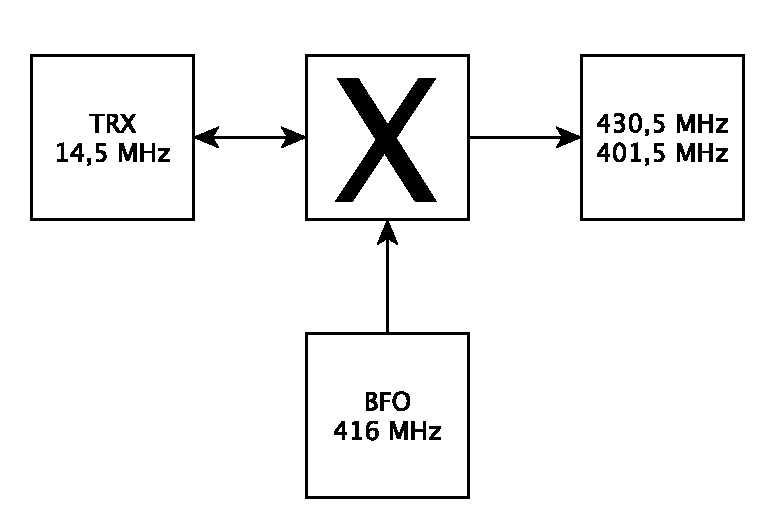
\includegraphics[width=1\textwidth,height=.6\textheight,keepaspectratio]{e15/transverter.pdf}
      \caption{Transverter}
    \end{figure}
  \end{center}
  Frequenzerweiterung für das Funkgerät. Hier: 20m auf 70cm.
\end{frame}

\section*{Empfänger}

\begin{frame}
  \frametitle{Direktüberlagerungsempfänger}
  Oder auch \emph{Superheterodynempfänger}, \emph{Superhet} oder \emph{Super}
  \begin{description}
    \item[super] \textit{(lat. super)} über
    \item[hetero] \textit{(griech. $\varepsilon\tau\varepsilon\rho o\varsigma$)} verschieden
    \item[dyn] \textit{(griech. $\delta\upsilon\nu\alpha\mu\iota\varsigma$)} Kraft
  \end{description}
  $\rightarrow$ Mischung zweier Signale unterschiedlicher Frequenz
\end{frame}

\begin{frame}
  \frametitle{Direktüberlagerungsempfänger -- Blockschaltbild}
  \begin{center}
    \begin{figure}
      \includegraphics[width=.99\textwidth]{e15/Ueberlagerungsempfanger_blockschaltbild.png}
      \attribcaption{Überlagerungsempfänger}{Appaloosa}{https://commons.wikimedia.org/wiki/File:Ueberlagerungsempfanger_blockschaltbild.svg}{\ccbysa}
    \end{figure}
  \end{center}
\end{frame}

\begin{frame}
  \frametitle{Spiegelfrequenz}
  \begin{center}
    \begin{figure}
      \includegraphics[width=.99\textwidth]{e15/Uberlagerungsempfanger_Spiegelfrequenz.png}
      \attribcaption{Spiegelfrequenz}{Znarf}{https://commons.wikimedia.org/wiki/File:Überlagerungsempfänger_Spiegelfrequenz.PNG}{\ccbysa}
    \end{figure}
  \end{center}
\end{frame}

\section*{Sonstiges}
\begin{frame}
  \frametitle{SNR}
  \begin{itemize}
    \item Das Signal-Rausch-Verhältnis dient als Bewertungszahl zur Beurteilung der Qualität eines (analogen) Kommunikationspfades.
    \item Um Sprache verstehen zu können braucht es ein SNR von ca 6dB.
  \end{itemize}
\end{frame}

\begin{frame}
  \frametitle{Trennschärfe}
  \begin{itemize}
    \item Beurteilt wie gut der Empfänger ein Signal von starken benachbarten Signalen trennen kann.
    \item Je steiler der Bandpass, desto besser die Trennschärfe.
  \end{itemize}
\end{frame}

\begin{frame}
  \frametitle{Großsignalfestigkeit}
  \begin{itemize}
    \item Beurteilt wie gut der Empfänger mit ganz starken Signalen zurechtkommt.
    \item Bekannt ist z.B. dann ein zugestopft des Empfängers bei zu starken Signalen (Erkennbar durch brummen).
  \end{itemize}
\end{frame}

\section*{Transceiver}

\begin{frame}
  \frametitle{BITX}
  \begin{figure}
    \includegraphics[width=.95\textwidth,height=.75\textheight,keepaspectratio]{e15/bitx-farbe.png}
      \caption{Schaltplan von \ExternalLink\url{http://www.phonestack.com/farhan/bitx.html}}
  \end{figure}
  6W SSB Transceiver für 14MHz
\end{frame}

\begin{frame}
  \frametitle{Elecraft - K3}
  \begin{center}
    \begin{figure}
      \includegraphics[width=1\textwidth,height=.75\textheight,keepaspectratio]{e15/K3_Front.jpg}
      \caption{Bild von \ExternalLink\url{http://www.elecraft.com/K3/K3.htm}}
    \end{figure}
  \end{center}
\end{frame}

\begin{frame}
  \frametitle{Drake TR-7}
  \begin{center}
    \begin{figure}
      \includegraphics[width=1\textwidth,height=.75\textheight,keepaspectratio]{e15/drake.jpg}
      \caption{Bild von DB4UM bei DK0TU}
    \end{figure}
  \end{center}
\end{frame}

\begin{frame}
  \frametitle{rad1o}
  \begin{center}
    \begin{figure}
      \includegraphics[width=1\textwidth,height=.75\textheight,keepaspectratio]{e15/rad1o.jpg}
      \caption{Bild von \ExternalLink\url{https://rad1o.badge.events.ccc.de/_media/rad1o_6.jpg}}
    \end{figure}
  \end{center}
\end{frame}

\begin{frame}
  \frametitle{rad1o -- Blockschaltbild}
  \begin{center}
    \begin{figure}
      \includegraphics[width=1\textwidth,height=.75\textheight,keepaspectratio]{e15/rad1o_block.pdf}
      \caption{Schaltplan von \ExternalLink\url{https://github.com/rad1o/hardware/blob/master/concept/overview_RF.pdf}}
    \end{figure}
  \end{center}
\end{frame}

\section*{Referenzen}

\begin{frame}
  \frametitle{Referenzen/Links}

  \footnotesize
  \begin{itemize}
    \item Moltrecht E 15: \\
      \url{https://www.darc.de/der-club/referate/ajw/lehrgang-te/e15/}
    \item Überlagerungsempfänger (Wikipedia): \\
      \url{https://de.wikipedia.org/wiki/\%C3\%9Cberlagerungsempf\%C3\%A4nger}
  \end{itemize}

\end{frame}

% Hier könnte noch eine Kontaktfolie stehen

\end{document}

